\section{eo\-Subtree\-XOver$<$ FType, Node $>$ Class Template Reference}
\label{classeo_subtree_x_over}\index{eoSubtreeXOver@{eoSubtreeXOver}}
eo\-Subtree\-XOver --$>$ subtree xover  


{\tt \#include $<$gp/eo\-Parse\-Tree\-Op.h$>$}

Inheritance diagram for eo\-Subtree\-XOver$<$ FType, Node $>$::\begin{figure}[H]
\begin{center}
\leavevmode
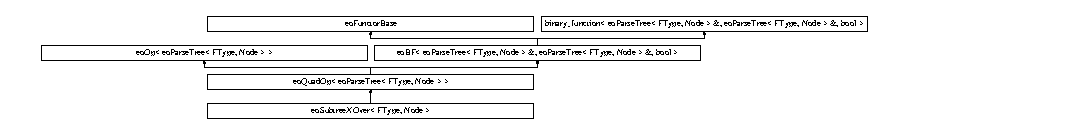
\includegraphics[height=1.36752cm]{classeo_subtree_x_over}
\end{center}
\end{figure}
\subsection*{Public Types}
\begin{CompactItemize}
\item 
typedef {\bf eo\-Parse\-Tree}$<$ FType, Node $>$ {\bf Eo\-Type}\label{classeo_subtree_x_over_w0}

\end{CompactItemize}
\subsection*{Public Member Functions}
\begin{CompactItemize}
\item 
{\bf eo\-Subtree\-XOver} (unsigned \_\-max\_\-length)
\begin{CompactList}\small\item\em Constructor. \item\end{CompactList}\item 
virtual std::string {\bf class\-Name} () const \label{classeo_subtree_x_over_a1}

\begin{CompactList}\small\item\em the ckassname \item\end{CompactList}\item 
virtual {\bf $\sim$eo\-Subtree\-XOver} ()\label{classeo_subtree_x_over_a2}

\begin{CompactList}\small\item\em Dtor. \item\end{CompactList}\item 
bool {\bf operator()} ({\bf Eo\-Type} \&\_\-eo1, {\bf Eo\-Type} \&\_\-eo2)\label{classeo_subtree_x_over_a3}

\begin{CompactList}\small\item\em Perform crossover on two individuals param \_\-eo1 The first parent individual param \_\-eo2 The second parent individual. \item\end{CompactList}\end{CompactItemize}
\subsection*{Private Attributes}
\begin{CompactItemize}
\item 
unsigned {\bf max\_\-length}\label{classeo_subtree_x_over_r0}

\end{CompactItemize}


\subsection{Detailed Description}
\subsubsection*{template$<$class FType, class Node$>$ class eo\-Subtree\-XOver$<$ FType, Node $>$}

eo\-Subtree\-XOver --$>$ subtree xover 



Definition at line 42 of file eo\-Parse\-Tree\-Op.h.

\subsection{Constructor \& Destructor Documentation}
\index{eoSubtreeXOver@{eo\-Subtree\-XOver}!eoSubtreeXOver@{eoSubtreeXOver}}
\index{eoSubtreeXOver@{eoSubtreeXOver}!eoSubtreeXOver@{eo\-Subtree\-XOver}}
\subsubsection{\setlength{\rightskip}{0pt plus 5cm}template$<$class FType, class Node$>$ {\bf eo\-Subtree\-XOver}$<$ FType, Node $>$::{\bf eo\-Subtree\-XOver} (unsigned {\em \_\-max\_\-length})\hspace{0.3cm}{\tt  [inline]}}\label{classeo_subtree_x_over_a0}


Constructor. 

\begin{Desc}
\item[Parameters:]
\begin{description}
\item[{\em \_\-max\_\-length}]the maximum size of an individual \end{description}
\end{Desc}


Definition at line 50 of file eo\-Parse\-Tree\-Op.h.

The documentation for this class was generated from the following file:\begin{CompactItemize}
\item 
eo\-Parse\-Tree\-Op.h\end{CompactItemize}
